% Sample paper for testing Paper Forge.
% It is deliberately written for the generic "article" class with natbib and
% geometry, so you can see Paper Forge move it onto the IEEE conference template.
\documentclass[11pt]{article}
\usepackage[margin=1in]{geometry}
\usepackage[numbers]{natbib}
\usepackage{graphicx}
\usepackage{amsmath}
\usepackage{booktabs}
\newcommand{\method}{\textsc{EdgeCache}}

\title{\method: Lightweight Result Caching for On-Device Neural Inference}
\author{Ada Example\\ Department of Computer Science, Example University\\ ada@example.edu
\and Brian Sample\\ Sample Research Lab\\ brian@sample.org}
\date{}

\begin{document}
\maketitle

\begin{abstract}
On-device neural inference is limited by latency and energy. We present \method{}, a lightweight cache
that reuses intermediate results for near-duplicate inputs. \method{} keys the cache on a locality-sensitive
hash of early-layer activations and falls back to full inference when the similarity is low. This sample
paper exists only to demonstrate Paper Forge; its numbers are illustrative, not real measurements.
\end{abstract}

\noindent\textbf{Keywords:} edge computing, caching, neural networks, inference latency

\section{Introduction}
\label{sec:intro}
Mobile and embedded devices increasingly run neural networks locally~\citep{lane2015early}. Many inputs seen by
such devices are near-duplicates: consecutive camera frames, repeated voice commands, or similar sensor
readings. Recomputing the full network for each input wastes time and energy.

We make three contributions: (1) a similarity key based on early activations, (2) a bounded cache with an
admission policy, and (3) an evaluation on illustrative workloads (Section~\ref{sec:eval}).

\section{Related Work}
Result caching for inference has been explored in cloud serving systems~\citep{crankshaw2017clipper}.
Model compression and pruning reduce cost per inference~\citep{han2016deep}, and are complementary to caching.

\section{Method}
\label{sec:method}
Given an input $x$, we compute the first $k$ layers to obtain activation $a_k(x)$ and its hash
\begin{equation}
h(x) = \operatorname{sign}(W a_k(x)), \quad W \in \mathbb{R}^{b \times d}.
\label{eq:hash}
\end{equation}
If a cached entry with Hamming distance below $\tau$ exists, its output is returned; otherwise the rest of the
network runs and the result is admitted according to Eq.~\eqref{eq:hash} and an LFU score.

\subsection{Admission Policy}
Entries are admitted when their predicted reuse probability exceeds a threshold. The threshold adapts to the
memory budget so the cache never exceeds a fixed size.

\section{Evaluation}
\label{sec:eval}
Figure~\ref{fig:latency} compares latency and Table~\ref{tab:results} summarizes accuracy. Values are
illustrative.

\begin{figure}[t]
\centering
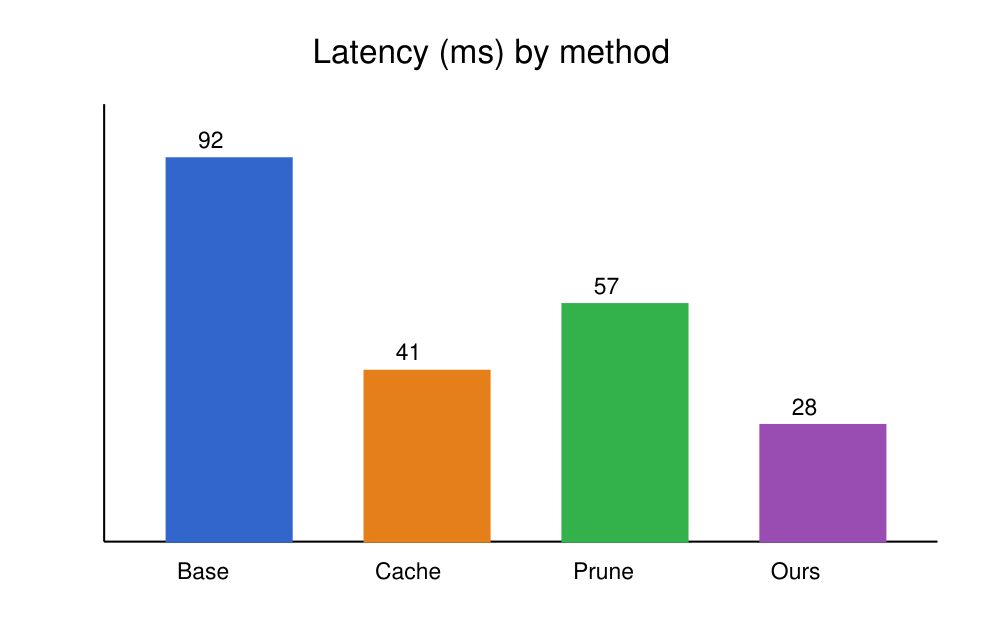
\includegraphics[width=0.9\linewidth]{figures/latency}
\caption{Mean inference latency per method (illustrative).}
\label{fig:latency}
\end{figure}

\begin{table}[t]
\centering
\caption{Accuracy and latency (illustrative values).}
\label{tab:results}
\begin{tabular}{lcc}
\toprule
Method & Top-1 (\%) & Latency (ms) \\
\midrule
Baseline & 76.1 & 92 \\
Pruning & 74.9 & 57 \\
\method{} & 75.8 & 28 \\
\bottomrule
\end{tabular}
\end{table}

Figure~\ref{fig:hitrate} shows the cache hit rate against standard policies.

\begin{figure}[t]
\centering
\includegraphics[width=0.9\linewidth]{hitrate.png}
\caption{Cache hit rate compared with classic policies (illustrative).}
\label{fig:hitrate}
\end{figure}

\section{Conclusion}
\method{} shows that simple result caching can cut on-device latency for near-duplicate inputs. Future work
includes learned similarity keys.

\section*{Acknowledgments}
This sample was written to test Paper Forge.

\bibliographystyle{plainnat}
\bibliography{references}
\end{document}
